\subsection{Topologie}
\label{subsec:CR:topologie}

Nous utilisons principalement deux topologies (A et B).

La topologie A est inspir� du \emph{testbed} de l'article de
R. Khalili \cite{pareto2013}, voir \fig{fig:topoMPTCP:A}. Nous avons
ajout�, � cette topologie, des routeurs priv�s entre le client et le
serveur \emph{MPTCP} pour disposer d'un nombre de sous-flots sup�rieur � deux.\\

\begin{figure}[!htb]
  \begin{changemargin}{-2.0cm}{0.5cm}
    \centering
    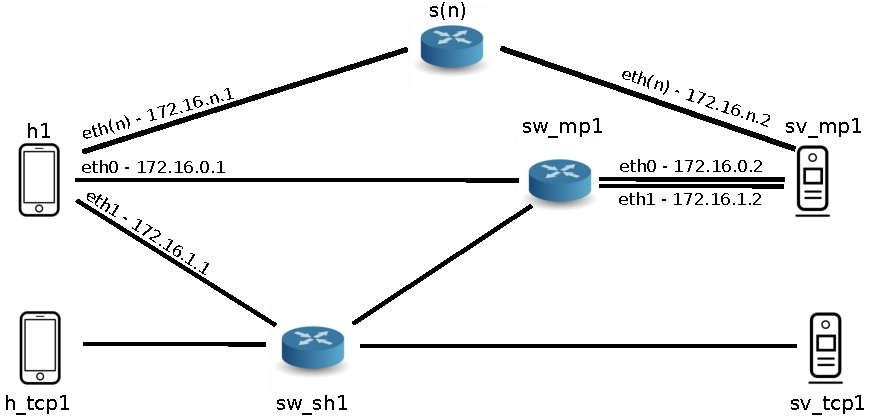
\includegraphics[width=0.7\textwidth]{../figures/mptcp_tcp/mptcp_tcp.pdf}
  \end{changemargin}
  \centering
  
  \caption{\textbf{Reproduction de la topologie de l'article de
      R. Khalili}. Le(s) \emph{switch(s)} ``S(n)'' ne sont pr�sent(s)
    que si le nombre de sous-flot est sup�rieure � deux. Pour n
    sous-flots, il y aura $n-2$ \emph{switchs} et $n-2$ liens
    suppl�mentaires. L'hyperviseur est connect� � tous les
    switchs. Pour se connecter via ssh aux h�tes, un \emph{switch} \og
    root \fg est cr�� et est connect� au \emph{switch} sw\_mp1 (non
    repr�sent� ici) voir utilisation CF linktobeadded.}
  \label{fig:topoMPTCP:A}
  
\end{figure}


La topologie B correspond au \emph{fat tree}.
